\chapter{System Analysis}

\section{Gantt Chart}
A Gantt chart represents the project schedule by mapping tasks against a timeline.
The SmartSec project was executed over 14 weeks, divided into ten structured phases.
Each phase builds upon the previous, ensuring stable and progressive implementation.

\begin{figure}[H]
    \centering
    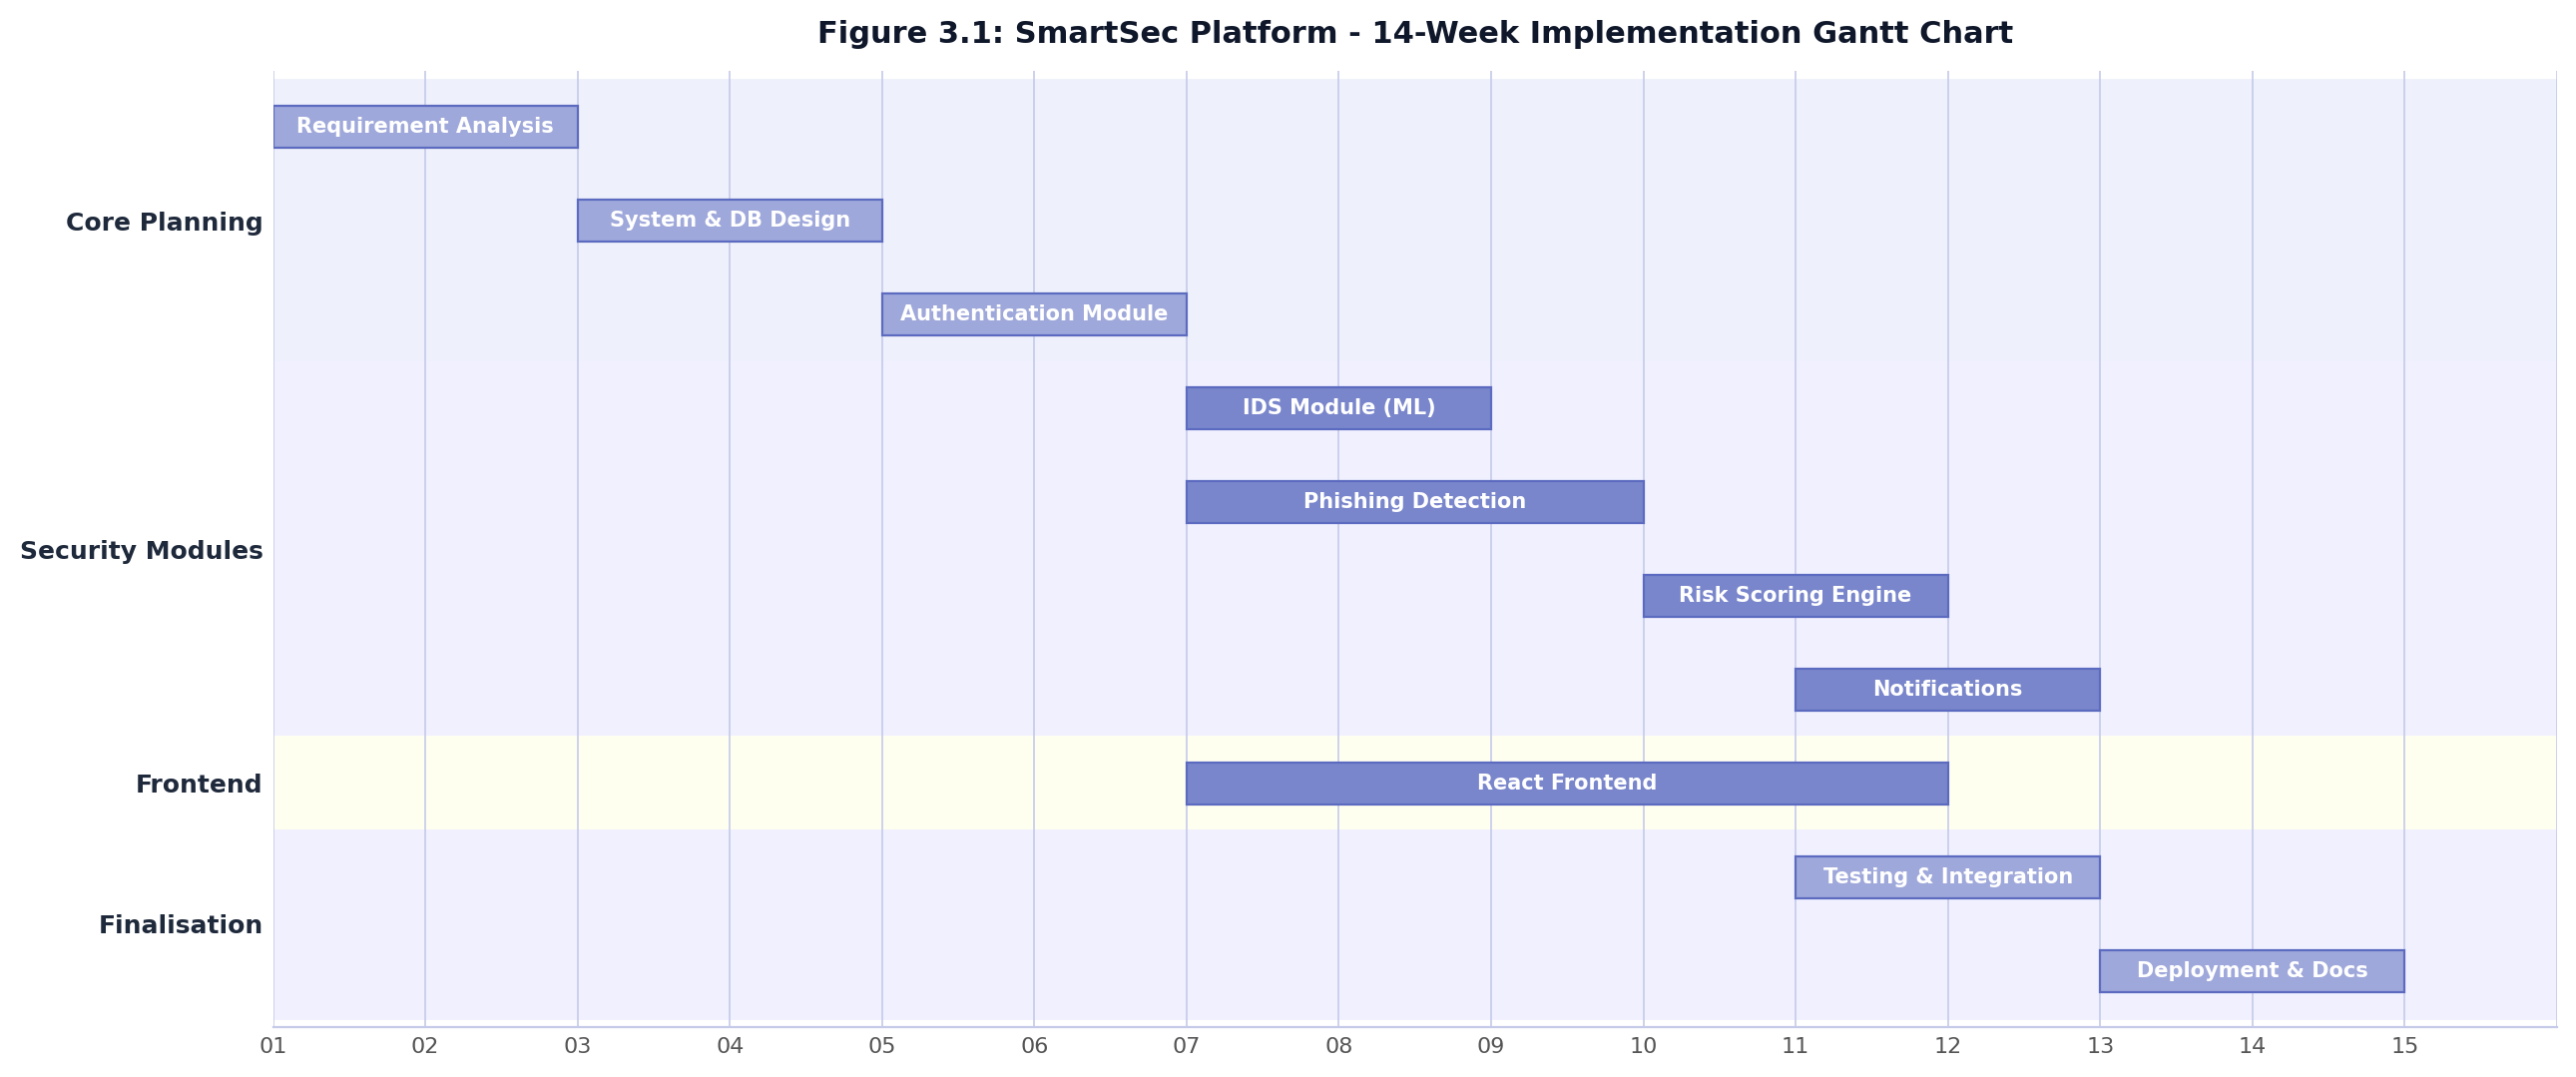
\includegraphics[width=1.0\linewidth]{gantt_chart}
    \caption{SmartSec Project Gantt Chart (14-Week Schedule)}
    \label{fig:gantt}
\end{figure}
\FloatBarrier

\noindent The phases covered are: Requirement Analysis (Weeks 1--2), System and Database Design (Weeks 3--4), Authentication Module (Weeks 5--6), IDS Module with ML model (Weeks 7--8), Phishing Detection Module (Weeks 7--9), Risk Scoring Engine (Weeks 9--10), Dashboard and Notifications (Weeks 10--11), React Frontend Development (Weeks 8--11), API Integration and Testing (Weeks 11--12), and Deployment and Documentation (Weeks 13--14).

\section{DFD Level 0 --- Context Diagram}
The DFD Level 0 (Context Diagram) shows the entire SmartSec system as a single process and illustrates its interactions with all external entities.

\begin{figure}[H]
    \centering
    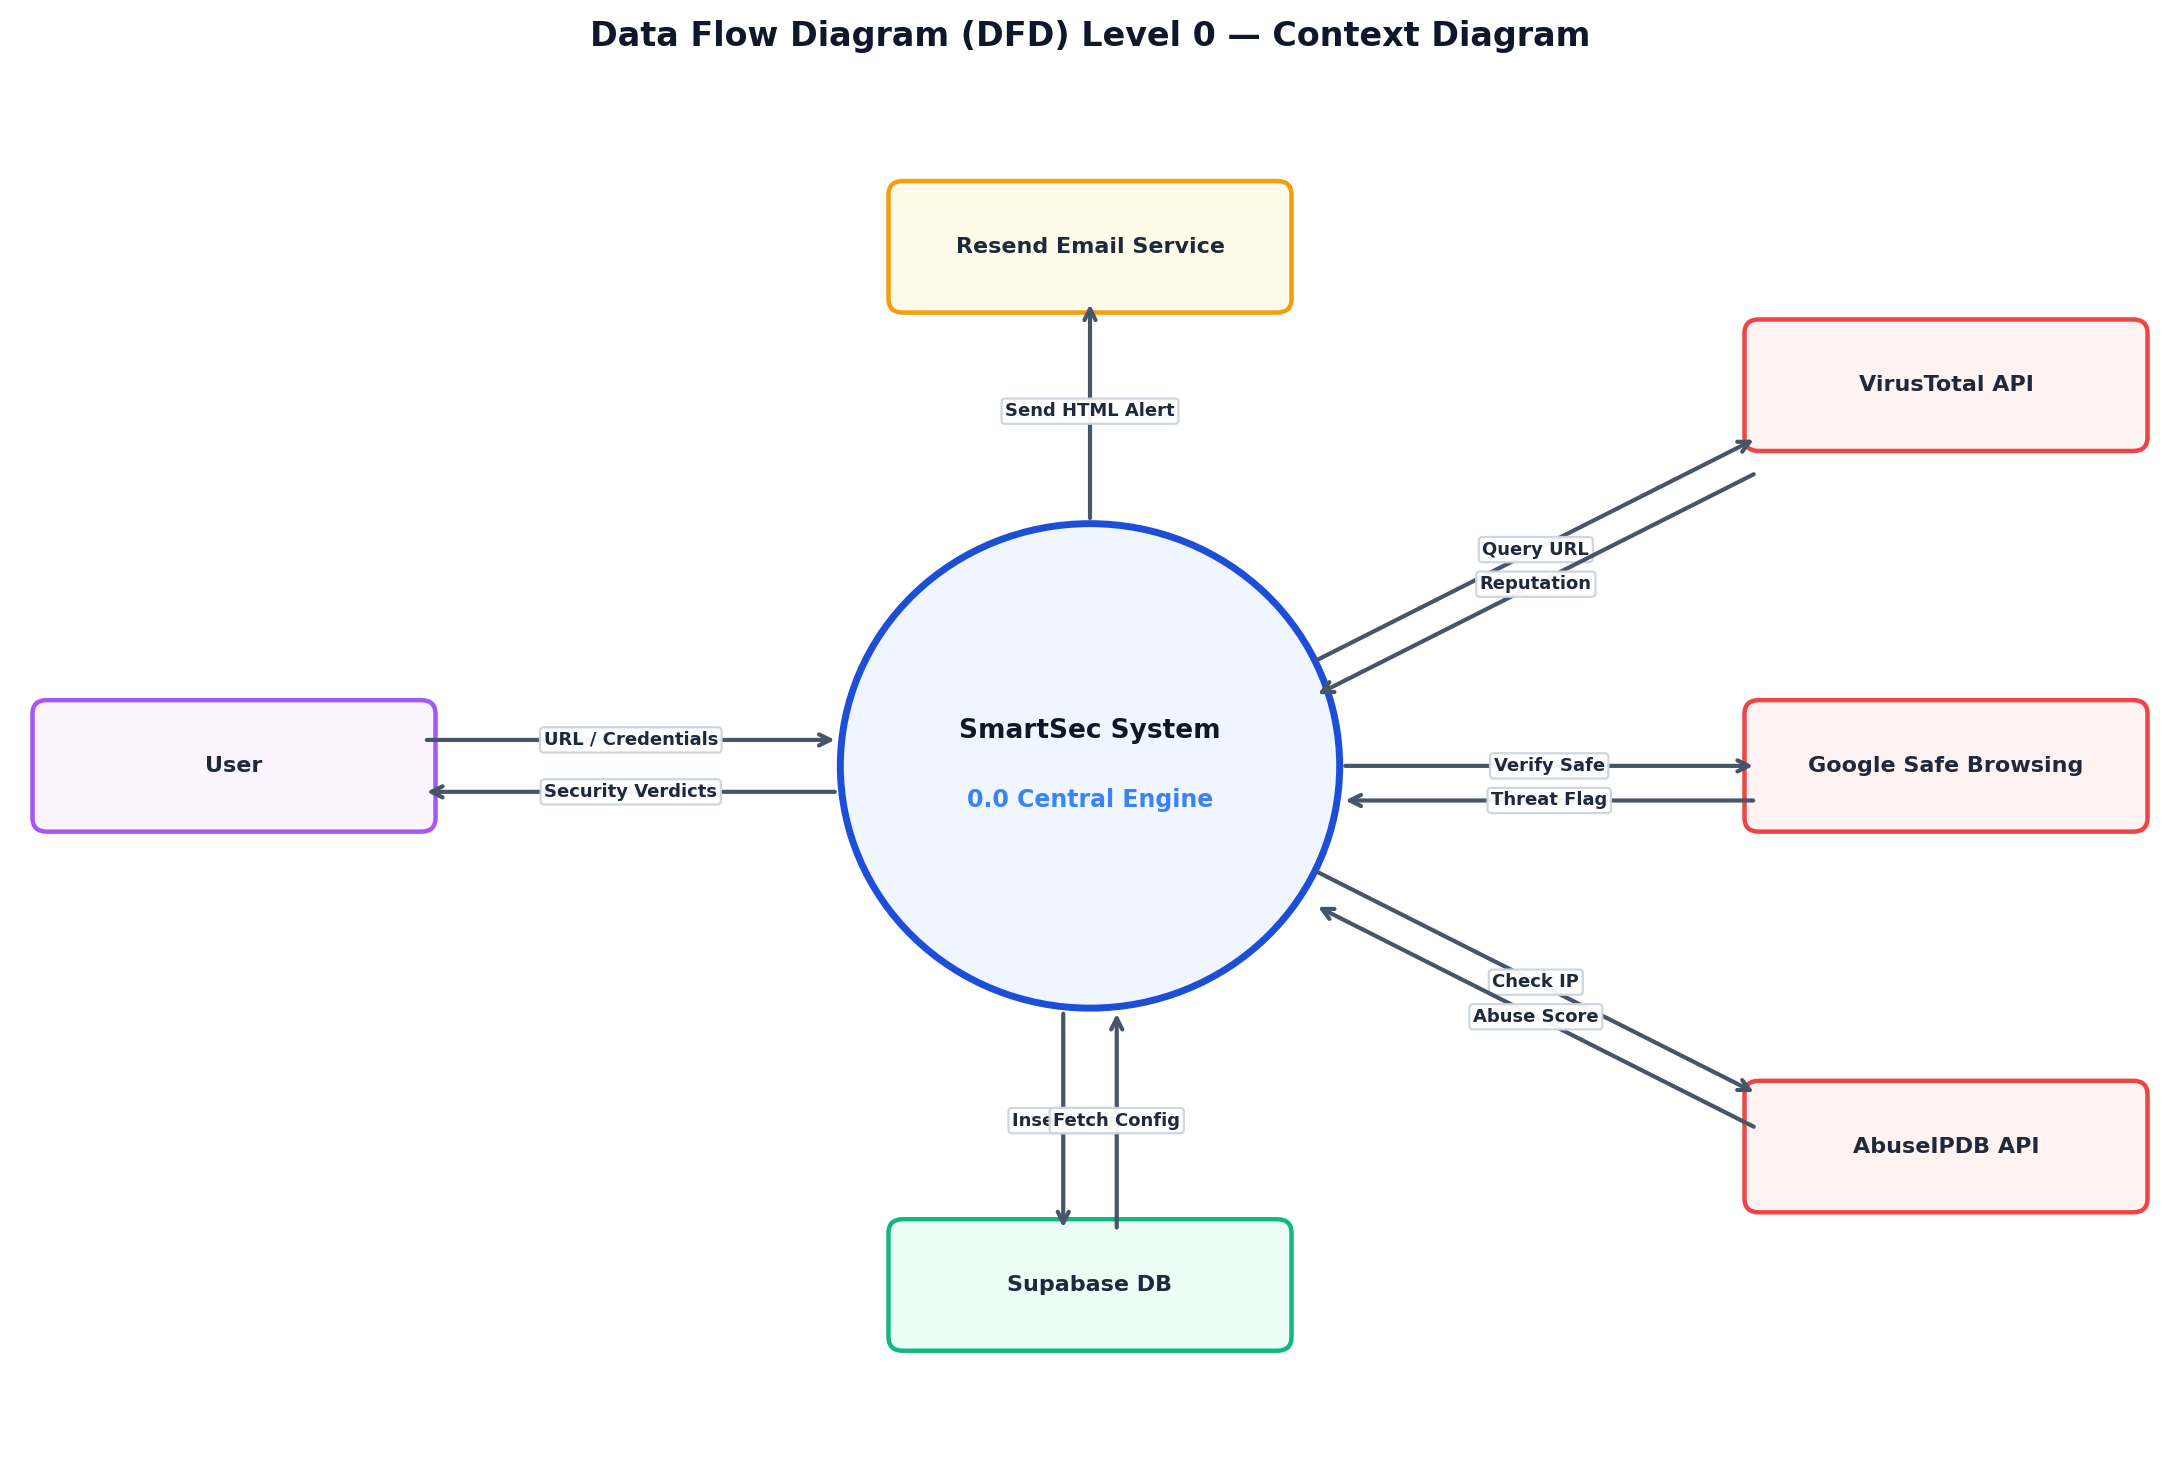
\includegraphics[width=0.95\linewidth]{dfd_level0}
    \caption{DFD Level 0 --- SmartSec System Context Diagram}
    \label{fig:dfd0}
\end{figure}
\FloatBarrier

\noindent The system interacts with seven external entities: \textbf{User} (submits credentials, URLs, and receives verdicts and notifications), \textbf{Supabase Database} (persists all security events and user data), \textbf{VirusTotal API} and \textbf{Google Safe Browsing API} (URL threat queries), \textbf{AbuseIPDB API} and \textbf{IPInfo API} (IP reputation and geolocation), and \textbf{Resend Email Service} (sends HTML alert emails for High and Critical events).

\section{DFD Level 1 --- Detailed Data Flow}
DFD Level 1 decomposes the central system process into six sub-processes, showing how data flows between them and the Supabase data stores.

\begin{figure}[H]
    \centering
    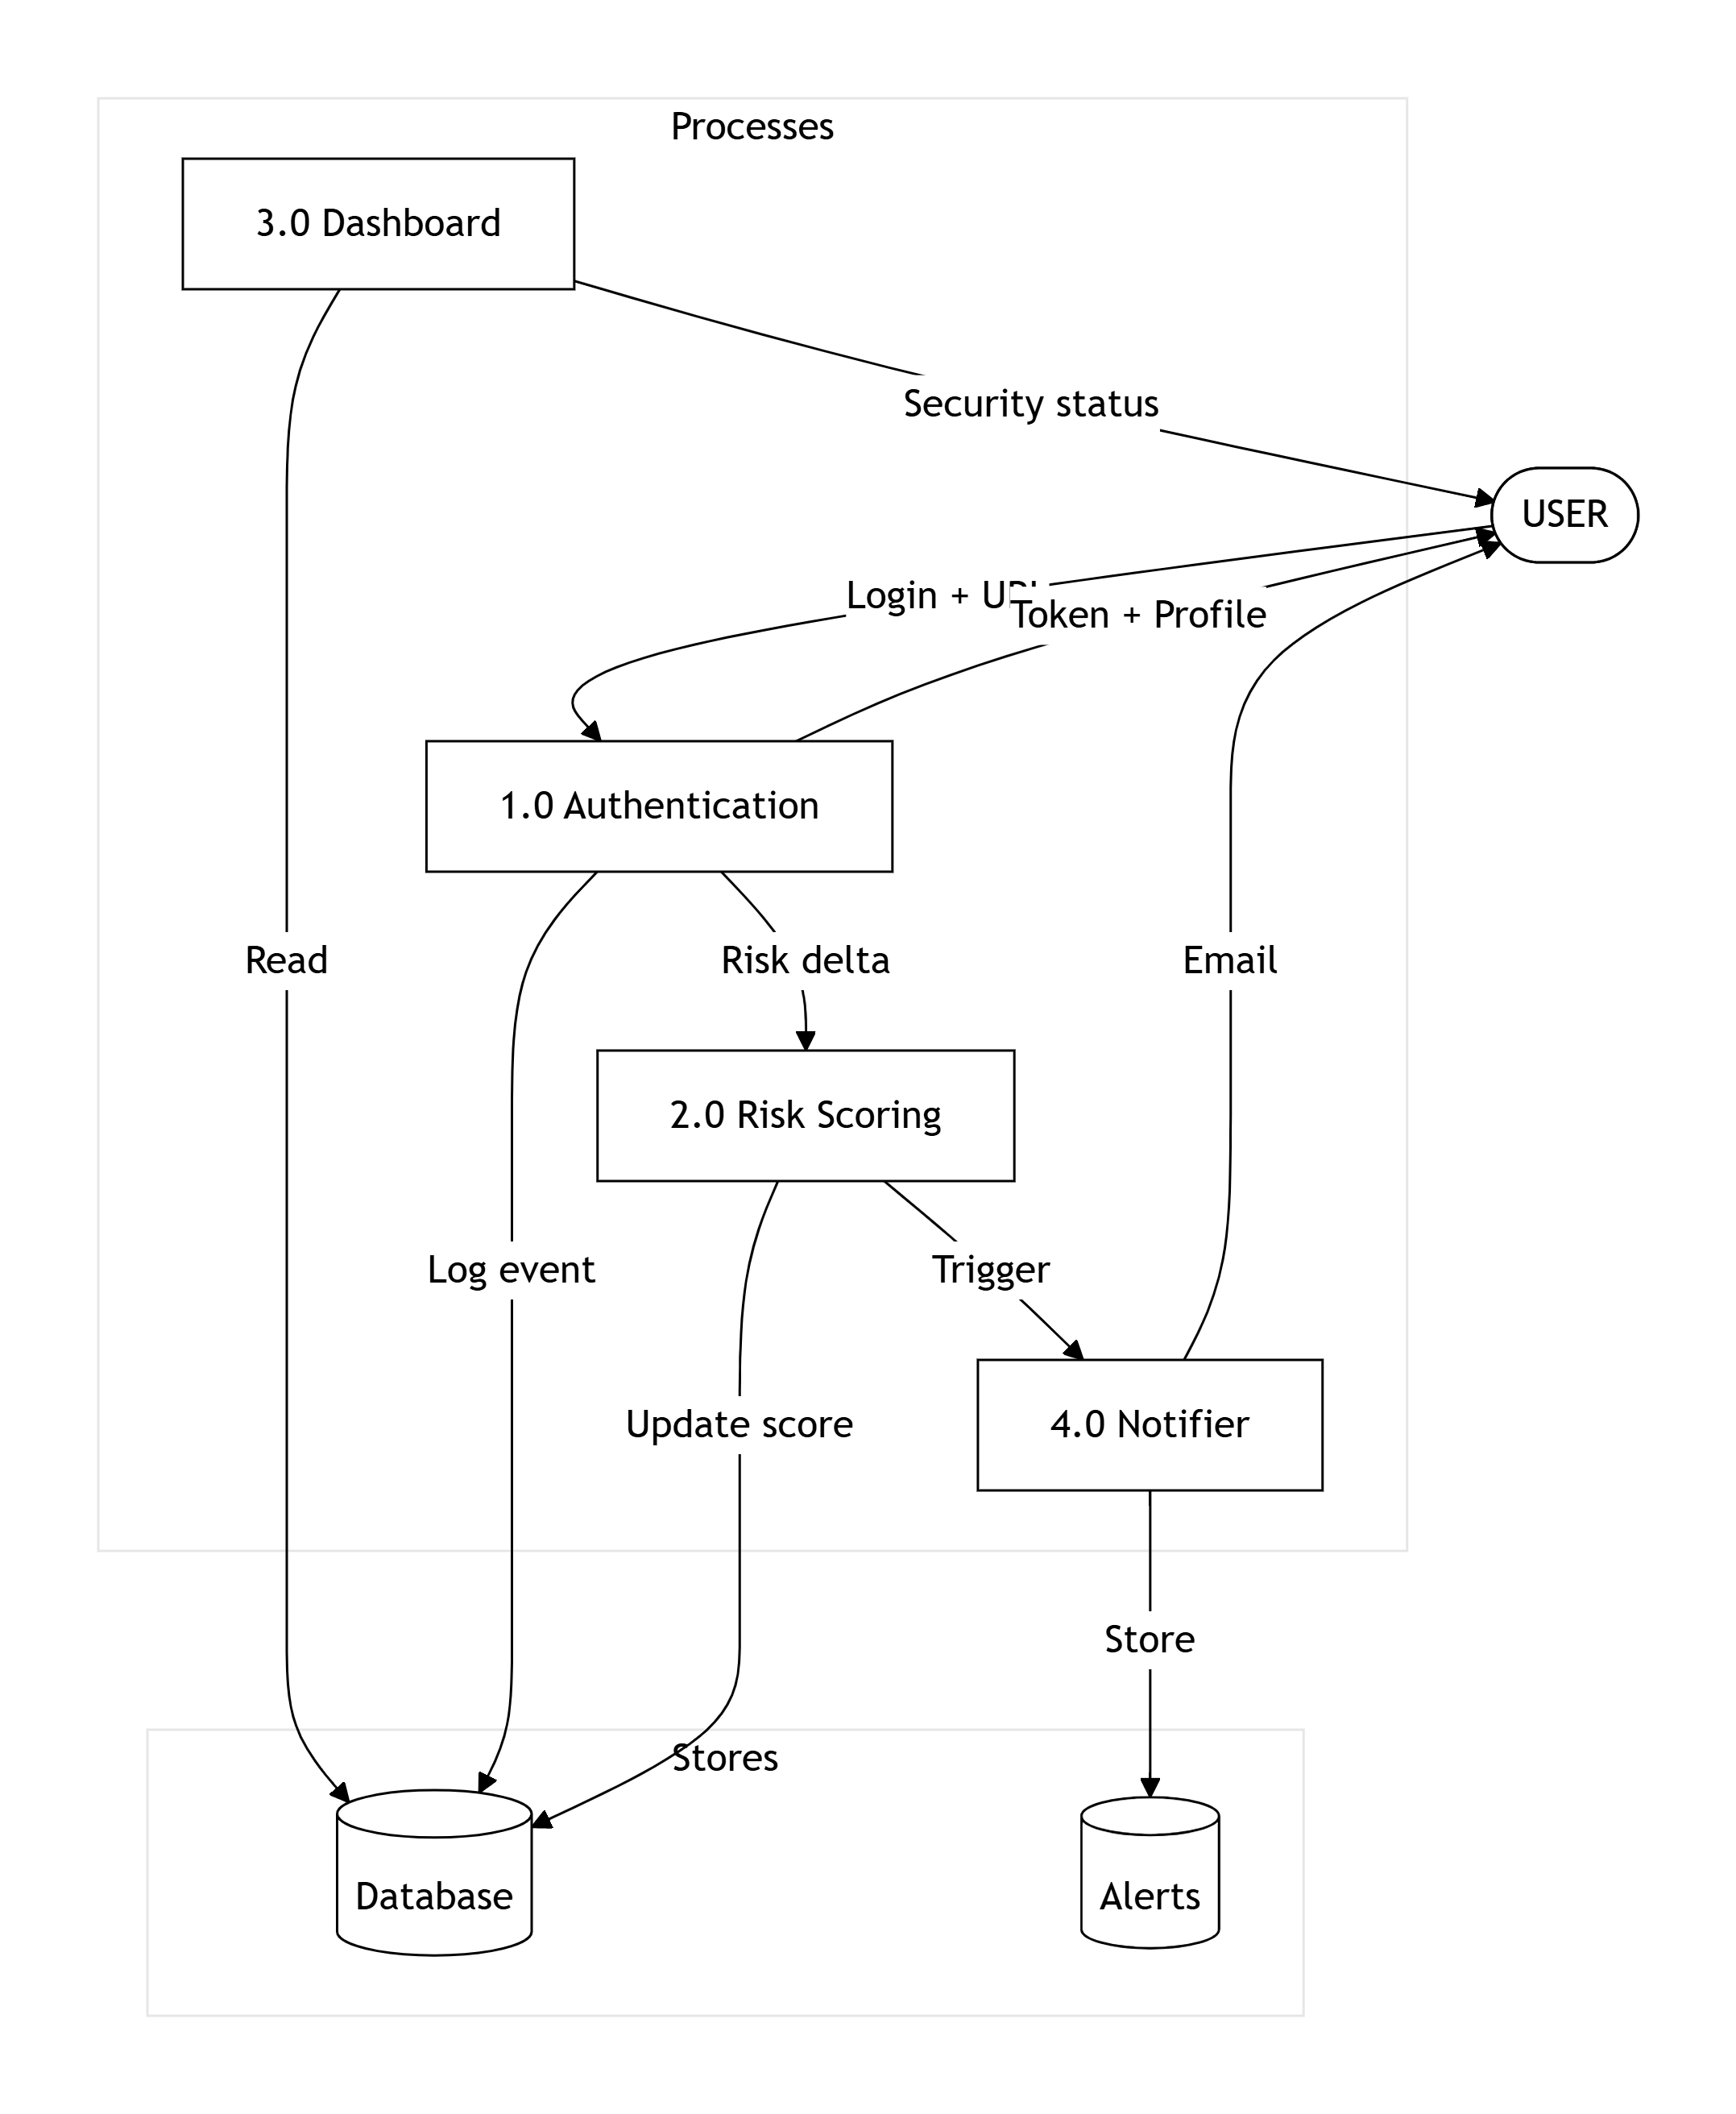
\includegraphics[width=\linewidth,height=0.75\textheight,keepaspectratio]{dfd1_new}
    \caption{DFD Level 1 --- Detailed Process and Data Flow Diagram}
    \label{fig:dfd1}
\end{figure}
\FloatBarrier

\noindent The six processes are: \textbf{1.0 Authentication} (handles login and registration, writes to D1 Users and D2 Login Events), \textbf{2.0 IDS Analysis} (runs IsolationForest inference, writes to D5 IDS Logs), \textbf{3.0 Phishing Detection} (multi-API URL analysis, writes to D3 URL Scans), \textbf{4.0 Risk Scoring} (calculates weighted decay score, writes to D4 Risk Events), \textbf{5.0 Dashboard Aggregation} (reads all stores to build dashboard response), and \textbf{6.0 Notification Delivery} (writes to D6 Notifications and triggers email alerts).

\section{Use Case Diagram}

\begin{figure}[H]
    \centering
    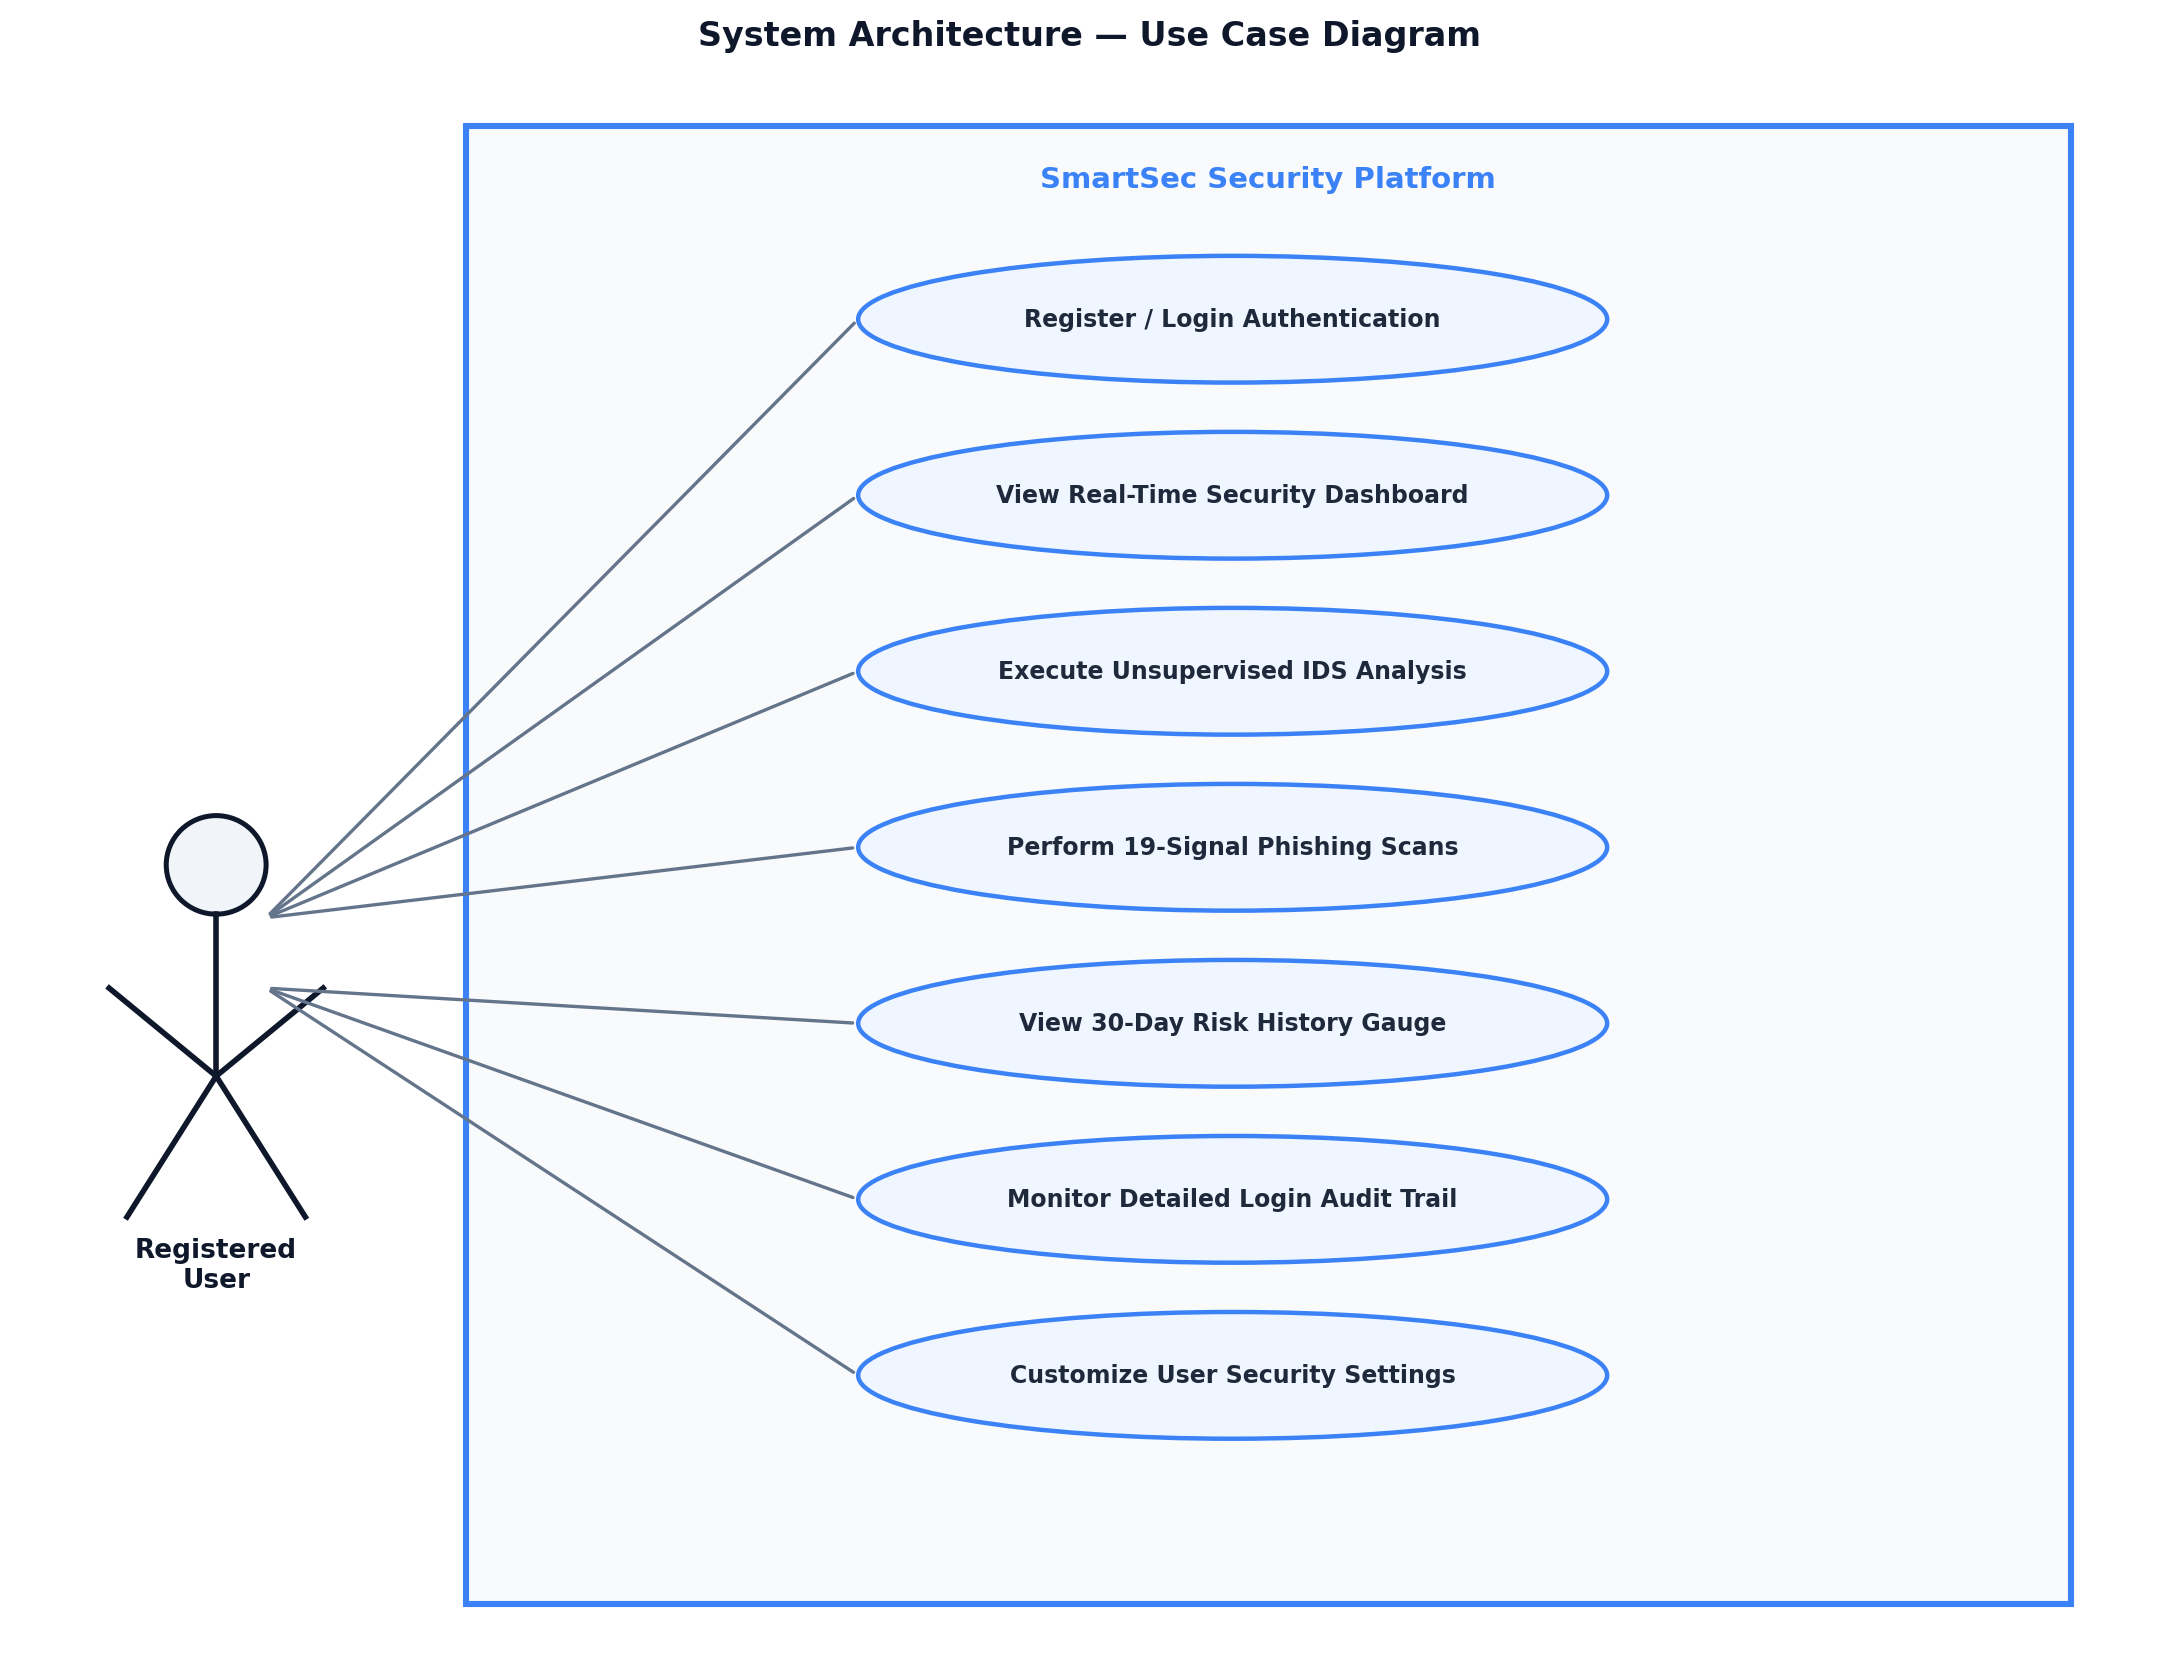
\includegraphics[width=0.85\linewidth]{usecase_diagram}
    \caption{SmartSec --- Use Case Diagram}
    \label{fig:usecase}
\end{figure}
\FloatBarrier

\noindent The Use Case Diagram identifies a single primary actor --- the registered \textbf{User} --- who interacts with nine use cases within the SmartSec system boundary: Register/Login, Scan URL for Phishing, Run IDS Analysis, View Security Dashboard, View Risk Score, View Login Activity, Manage Profile, Configure Settings, and View Notifications.

\section{Operating Tools and Technology}

\subsection*{Hardware Requirements}
\begin{itemize}
    \item Processor: Intel Core i5 or higher (Core i7 recommended for ML model training)
    \item RAM: Minimum 8 GB (16 GB recommended)
    \item Storage: At least 10 GB free disk space
    \item Internet Connection: Required for all external API integrations
\end{itemize}

\subsection*{Software Requirements}
\begin{itemize}
    \item Operating System: Windows 10 / Ubuntu 22.04 LTS or newer
    \item Backend: Python 3.11+, FastAPI 0.111+, Uvicorn ASGI server
    \item Machine Learning: scikit-learn 1.5+ (IsolationForest), NumPy 2.0+
    \item Database: PostgreSQL 15+ via Supabase hosted platform
    \item Frontend: Node.js 18+, React 18, Vite 5, Vanilla CSS, Recharts
    \item Threat APIs: VirusTotal v3, Google Safe Browsing v4, AbuseIPDB, IPInfo
    \item Email: Resend API; Authentication: python-jose (JWT), passlib (bcrypt)
    \item Deployment: Docker + Render.com (backend), Vercel (frontend)
    \item IDE: Visual Studio Code; Browser: Google Chrome
\end{itemize}
